\input{mmd-article-header}
\def\mytitle{BOSH Technical Overview}
\def\myauthor{VMware 2012 - Cloud Foundry}
\def\latexmode{memoir}
\input{mmd-article-begin-doc}
\chapter{Introduction}
\label{introduction}

BOSH (\textbf{B}osh \textbf{O}uter \textbf{SH}ell) is an automation framework that allows a small ops team to manage components and deployments. BOSH is called the ``outer shell'' because it provisions virtual machines inside an ``inner shell,'' the group of services that need to be deployed\slash maintained in your cloud. In VMware’s case, Cloud Foundry is the inner shell that BOSH deploys.

\chapter{Background}
\label{background}

Manually creating an application cloud (VMware’s case) is a lot of work. Virtual Machines (VMs) must be provisioned, software prerequisite packages must be installed (ruby, gems, jvm, rabbitmq, mysql, libraries, etc.), application cloud services must be deployed (router, application scheduling system, health manager, VM controlling agents), and network\slash shared components (nfs, amqp, networking, dns, etc.) must be configured. There is also maintenance work. Performing updates is inherently more complex than the initial deployment because the ops team has to minimize the disruption to any running customers’ applications, deal with data migrations\slash rollbacks in case the update had a critical issue, and take into account different component versions.

\chapter{Features and Benefits}
\label{featuresandbenefits}

The outer shell should automate all of the common tasks on the inner shell for the ops team.

\begin{itemize}
\item \textbf{Automated Deployments} - It should allow the ops team to deploy the inner shell without manually setting up each VM (cloning, network settings, etc), installing the required packages, or configuring the components individually.

\item \textbf{Automated Updates} - It should allow the ops team to update the inner shell in a reliable way.

\item \textbf{Ops Tools} - It should provide tools that enable the ops team to deal with unexpected production issues. Tools such as rollbacks, data migrations, traffic monitoring, automated alerting etc.

\item \textbf{Reliable\slash Easy to Use} - The above operations should be as painless as possible so the ops team can push often and reliably. They should not be afraid of performing a rollback in case something goes wrong. Also, updates should have the least impact on the customers’ running applications, which means rolling updates and enabling components to drain their traffic.

\item \textbf{Service Scalability} - It should provide an easy mechanism for the ops team to scale each service up or down based on demand. Infrastructure\slash Version Scalability - It should support multiple instances of AppCloud in multiple data centers and should efficiently enable version diversity across a pool of AppCloud instances.

\item \textbf{Infrastructure Portability} - It should support many IaaS using an abstraction layer to manage VMs and templates so that the difference between Redwood, vSphere, AWS is simply a configuration file.

\end{itemize}

On top of this, the ideal is to have updates happen frequently (once per week) to support an agile development model.

\section{Assumptions about IaaS}
\label{assumptionsaboutiaas}

BOSH was built to assist operations staff in provisioning and maintaining virtual machines on top of Infrastructure as a Service such as VMWare vSphere, or Amazon EC2. In order for BOSH to perform its role, certain assumptions are made about this layer underneath.

\begin{itemize}
\item IaaS will gracefully handle physical failures by restarting VMs on a different host when failures occur.

\item IaaS will provide some sort of placement so outer shell will not have to place VMs onto specific physical host.

\item IaaS will provide persistent storage.

\end{itemize}

\section{Simple Deployment Example using BOSH}
\label{simpledeploymentexampleusingbosh}

\begin{adjustwidth}{2.5em}{2.5em}
\begin{verbatim}

# Set bosh commands to point at the director.
bosh target http:   //your.director.address:8080

# Upload your stemcell (base VM) for all new VMs to use.
bosh upload stemcell bosh-stemcell.tgz

# Create a release -- this pulls from a configured repository
cd ~/release
./update
bosh create release

# Upload the release
bosh upload release releases/cloudfoundry-1.yml

# Set Bosh to use this configuration file for the inner shell deployment.
bosh deployment path/to/deployment.yml

# Deploy the inner shell.
bosh deploy

\end{verbatim}
\end{adjustwidth}

\chapter{Components}
\label{components}

The outer shell contains or interacts with: \textbf{director}, \textbf{health monitor}, \textbf{tsdb}, \textbf{nats}, \textbf{blobstore}, and \textbf{datastore}.

\begin{table}[htbp]
\begin{minipage}{\linewidth}
\setlength{\tymax}{0.5\linewidth}
\centering
\small
\begin{tabulary}{\textwidth}{@{}CL@{}} \toprule
Component&Description\\
\midrule
\textbf{director}&Responsible for all operations done on inner shell services, such as setup, updates, roll backs, take down, etc. Also provides a REST API for operators to perform these action\\
\textbf{agent}&Receives commands from the director through its own API. (This component is in the inner shell)\\
\textbf{health monitor}&Constantly monitors services running in the inner shell (using the inner shell agents). If it finds any problems, it may notify the tsdb and director so that alerts can be fired, triggering an action by the director.\\
\textbf{tsdb}&Monitoring aggregation service. Collects stats about the inner shell services and provides tools for ops such as graphs and automated alerting.\\
\textbf{nats}&Not A Typical Service. A central message bus. All communications between outer shell and inner shell components are routed through it.\\
\textbf{blobstore}&Holds VM templates (stemcells), source packages, and compiled packages for inner shell deployments.\\

\midrule
\textbf{datastore}&Holds metadata about inner shell deployments.\\

\bottomrule

\end{tabulary}
\end{minipage}
\end{table}


\section{Figure 1. Interaction of BOSH Components}
\label{figure1.interactionofboshcomponents}

An illustration of how BOSH creates and manages virtual machines within an IaaS.

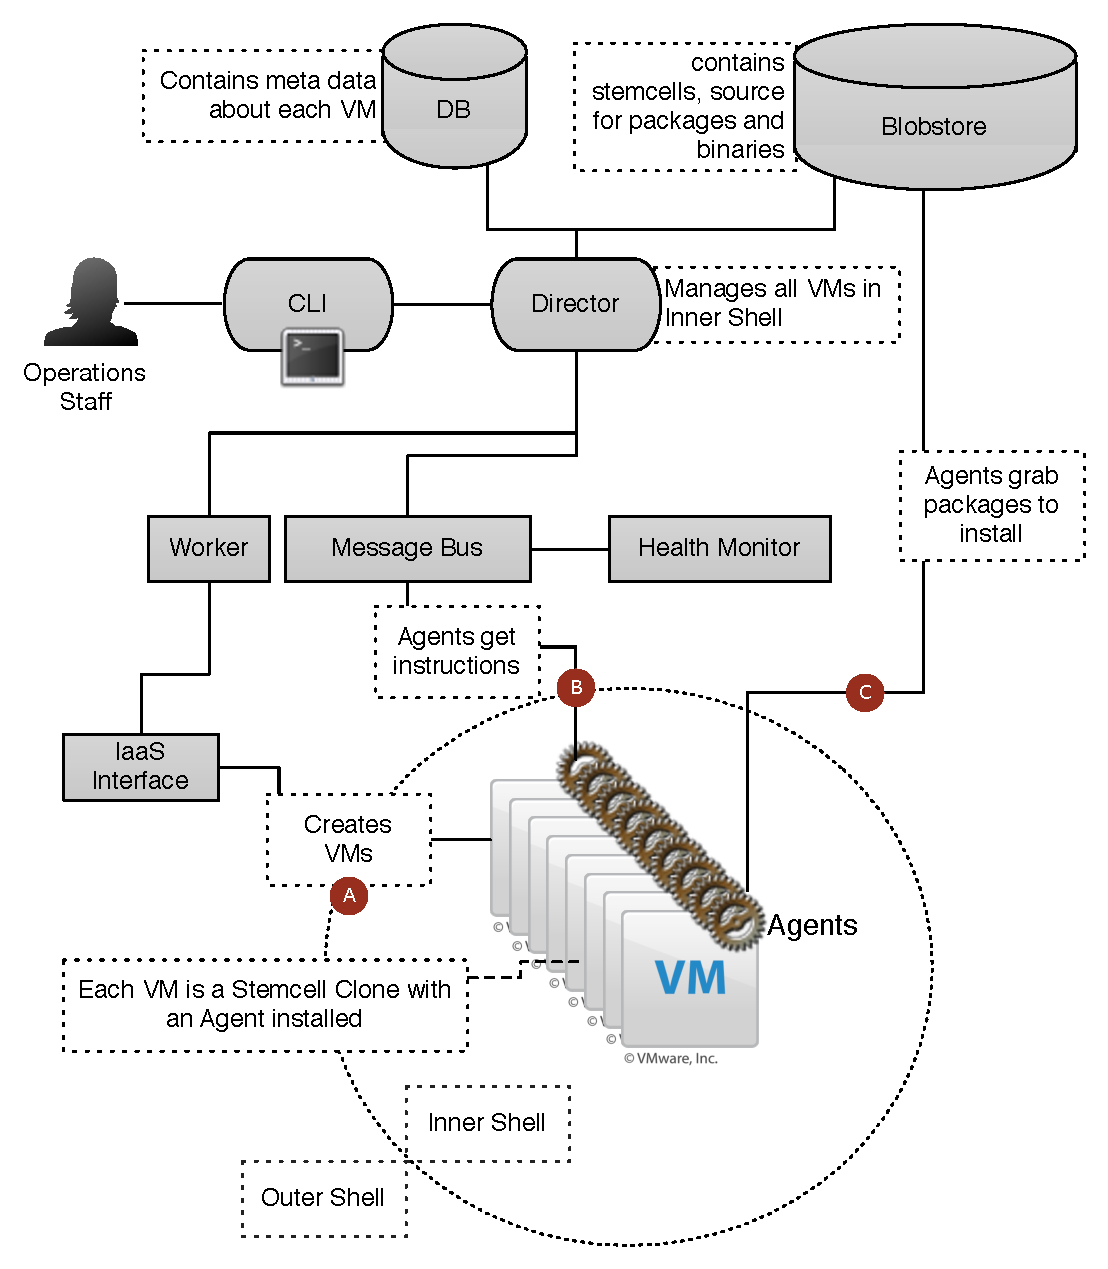
\includegraphics[keepaspectratio,width=\textwidth,height=0.75\textheight]{fig1.pdf}


\section{Inner Shell Deployment}
\label{innershelldeployment}

An inner shell deployment is initiated by an operator using the BOSH command line tool and is run by the Director. In order for the director to know how something about the VMs to create, it is passed a configuration file. The sequence of events is as follows:

\begin{enumerate}
\item Operations staff uses CLI to send config to Director with bosh deploy

\item Director compares (diff) Config with metadata to understand what it needs to create

\item Director creates VMs and sends instructions to VM

\item VMs are created from stemcells

\end{enumerate}

\section{Figure 2. Inner Shell Deployment}
\label{figure2.innershelldeployment}

The following is an Illustration of the events listed on the previous page. 

\begin{figure}[htbp]
\centering
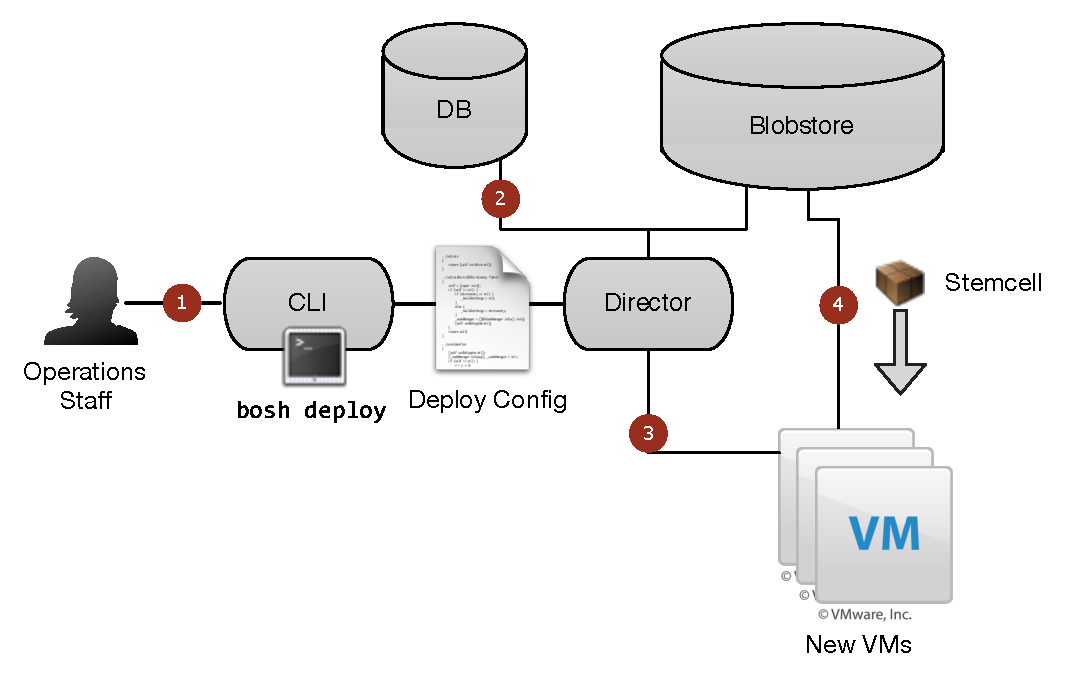
\includegraphics[keepaspectratio,width=\textwidth,height=0.75\textheight]{fig2.pdf}
\caption{image}
\label{}
\end{figure}



\chapter{Deployment Configuration}
\label{deploymentconfiguration}

The deployment config shown in Figure 2. is the top level configuration for an inner shell deployment. It is used to specify what you would like to deploy. In it, you name the jobs (Ex: MySQL Customer DB) for each VM, how many instances of them should be created, the resources they should get (RAM, disk, CPU), network configuration, and properties such as user\slash pass. An example of a configuration file appears in section 5.2.

\section{Sections of a Deploy Config}
\label{sectionsofadeployconfig}

\begin{table}[htbp]
\begin{minipage}{\linewidth}
\setlength{\tymax}{0.5\linewidth}
\centering
\small
\begin{tabulary}{\textwidth}{@{}CL@{}} \toprule
Item&Description\\
\midrule
\textbf{name}&a unique name for the deployment, which allows multiple deployments\\
\textbf{release information}&tells the director which release version the deployment should be running\\
\textbf{networks}&network pools for this deployment (\texttt{cloud\_properties}) are arguments passed to the Cloud Provider so it can properly configure the VM networking)\\
\textbf{resource pools}&a profile that is assigned to a job which describes things such as what stemcell should be used and how much RAM\slash CPU\slash disk the VM should be given\\
\textbf{update settings}&defines the characteristics of how updates are performed. It specifies how many instances of a job should be updated at the same time, what is the max threshold of errors before an automatic revert is applied, and how many instances should be checked for successful updates and for how long. In BOSH this check is performed by a beacon known as a Canary\\
\textbf{job specifications}&the specifications for a job, such as the network addresses, which resource pool profile it uses, how many instancesshould run, and how much persistent disk it should have\\

\bottomrule

\end{tabulary}
\end{minipage}
\end{table}


\section{An incomplete config example}
\label{anincompleteconfigexample}

\begin{adjustwidth}{2.5em}{2.5em}
\begin{verbatim}

name: staging
director_uuid: 374d1703-c744-42e5-a773-9299c3f1d1a1
release:
  name: my_cloud
  version: 3
networks:
- name: databases
  subnets:
  - static:
    - 172.23.2.17 - 172.23.2.128
    range: 172.23.2.0/23
    gateway: 172.23.2.1
    dns:
    - 172.22.22.153
    - 172.22.22.154
    cloud_properties:
      name: VLAN2002
resource_pools:
- name: small
  stemcell:
    name: bosh-stemcell
    version: 0.3.1
  network: management
  size: 15
  cloud_properties:
    ram: 1024
    disk: 4096
    cpu: 1
update:
  canaries: 1
  canary_watch_time: 15000
  update_watch_time: 15000
  max_in_flight: 1
  max_errors: 1
jobs:
- name: mysql_employee_instance
  template: mysql_employee
  instances: 1
  resource_pool: small
  persistent_disk: 32768
  networks:
  - name: databases
    static_ips:
    - 172.23.8.21

\end{verbatim}
\end{adjustwidth}

\section{Release Deployment}
\label{releasedeployment}

When an inner shell deployment is done the jobs must be started on a VM that has their required packages (such as Redis, nginx, MySQL, etc.). A ``release'' is the way all packages for a deployment are uploaded to the blobstore. When an inner shell deployment is done, a release version is specified, indicating which packages (and what versions of them) should be used.

A release bundle is an archive containing packages, job manifests, and a release manifest. There is a configuration file for each versioned release, which contains a list of versioned packages and jobs that should be part of a release. After a release has been uploaded, the inner shell deployment configuration is changed so that the next deployment will use the new release.

\section{Example of Release Deployment}
\label{exampleofreleasedeployment}

\begin{adjustwidth}{2.5em}{2.5em}
\begin{verbatim}

--- 
packages:
- name: mongodb_node
  version: 25
  sha1: 89ea5fd41c9f85bd8ba3f2782ae6759707af30c3
  dependencies: 
  - sqlite
  - ruby
- name: mysql
  version: 4
  sha1: 6f2420a6a0d654b64146294a4b43bcd75c8c958d
  dependencies: []
- name: mysql_gateway
  version: 25
  sha1: cfb492b94068c890a028a6798d2f02361a28f2e8
  dependencies: 
  - mysqlclient
  - sqlite
  - ruby
- name: mysql_node
  version: 25
  sha1: 4df13f3f35ef56f98dd1ebf319b47b51a9911fe5
  dependencies: 
  - mysqlclient
  - sqlite
  - ruby
- name: mysqlclient
  version: 1
  sha1: 66db38d9a0e6c1e76d0e7bf1d12b29546f0ac74d
  dependencies: []

\end{verbatim}
\end{adjustwidth}

\section{Package Configuration}
\label{packageconfiguration}

A package is a compressed tarball consisting of some application code, a package manifest in YAML format, and a set of migrations (if any) that need to be run when upgrading an existing component. Packages cannot contain binaries because the deployment target might not match the characteristics (32bit vs 64bit, library versions, etc..) of the ``build'' machine. The package manifest consists of a name, version, script to compile the package, and migration scripts for migrating existing data when a package is installed.

A package is built from a package spec, also in YAML formal, that consists of metadata and a list of files that describe the contents of the package.

\section{Example Package Config}
\label{examplepackageconfig}

Contents of \texttt{packages\slash cloudcontroller.pkg}:

\begin{center}\rule{3in}{0.4pt}\end{center}


\begin{adjustwidth}{2.5em}{2.5em}
\begin{verbatim}

---
name: cloudcontroller
packaging:  packages/cloudcontroller/packaging
migrations: packages/cloudcontroller/migrations
files:
- cloudcontroller/**/*

\end{verbatim}
\end{adjustwidth}

\begin{center}\rule{3in}{0.4pt}\end{center}


Contents of \texttt{packages\slash cloudcontroller\slash packaging}:

\begin{center}\rule{3in}{0.4pt}\end{center}


\begin{adjustwidth}{2.5em}{2.5em}
\begin{verbatim}

#!/usr/bin/env bash
bundle install vendor

\end{verbatim}
\end{adjustwidth}

\begin{center}\rule{3in}{0.4pt}\end{center}


Contents of \texttt{packages\slash rabbitmq.pkg}:

\begin{center}\rule{3in}{0.4pt}\end{center}


\begin{adjustwidth}{2.5em}{2.5em}
\begin{verbatim}

---
name: rabbitmq
packaging: packages/rabbitmq/packaging
files:
- rabbitmq-server-1.8.0.tar.gz

\end{verbatim}
\end{adjustwidth}

\begin{center}\rule{3in}{0.4pt}\end{center}


Contents of \texttt{packages\slash rabbitmq\slash packaging}:

\begin{center}\rule{3in}{0.4pt}\end{center}


\begin{adjustwidth}{2.5em}{2.5em}
\begin{verbatim}

#!/usr/bin/env bash
tar xzf rabbitmq-server-1.8.0.tar.gz
cd rabbitmq-server-1.8.0
make

\end{verbatim}
\end{adjustwidth}

\begin{center}\rule{3in}{0.4pt}\end{center}


Packages are copied to the stem cell VMs and are stored in \texttt{\slash bosh\slash packages\slash $<$package name$>$\slash $<$package version$>$\slash } and the contents will not be writable.

\chapter{Jobs}
\label{jobs}

A job is composed of one or more packages and describes what the director\slash agent should deploy and monitor. A stem cell will take on a role of a single job and will be deleted once the job is no longer needed.

The job is described by a job manifest, Monit script, configuration script, lifecycle hooks, and required packages.

\section{Example Job Manifest}
\label{examplejobmanifest}

This is an example manifest for a job named \texttt{cloud\_controller}. The manifest lists all of the configuration templates, many of which are Embedded Ruby \texttt{.erb} files, containing variables that will be processed when the configuration file is created. The bottom of the file lists the packages that must be downloaded installed on the stemcell to create the Virtual Machine and turn it into this job (role). Contents of
\texttt{jobs\slash cloudcontroller\slash spec}:

\begin{center}\rule{3in}{0.4pt}\end{center}


\begin{adjustwidth}{2.5em}{2.5em}
\begin{verbatim}

---
name: cloud_controller
templates:
  nginx_ctl:      bin/nginx_ctl
  nginx.conf.erb:     config/nginx.conf
  mime.types:     config/mime.types
  cloud_controller.yml.erb: config/cloud_controller.yml
  cloud_controller_ctl.erb: bin/cloud_controller_ctl
  nfs-common: config/nfs-common
  idmapd.conf.erb: config/idmapd.conf
  node_staging.yml: config/staging/node.yml
  sinatra_staging.yml: config/staging/sinatra.yml
  java_web_staging.yml: config/staging/java_web.yml
  spring_staging.yml: config/staging/spring.yml
  rails3_staging.yml: config/staging/rails3.yml
  grails_staging.yml: config/staging/grails.yml
  lift_staging.yml: config/staging/lift.yml
  platform_staging.yml: config/staging/platform.yml
  sudoers: config/sudoers
  blacklist.txt: config/blacklist.txt
  syslog_forwarder.conf.erb: config/syslog_forwarder.conf
  iptables.conf.erb: config/iptables.conf
packages:
  - cloud_controller
  - libpq
  - sqlite
  - mysqlclient
  - ruby
  - syslog_aggregator
  - nginx
  - insight_agent

\end{verbatim}
\end{adjustwidth}

\chapter{Stem Cells}
\label{stemcells}

Stem Cells{\ldots} write about this.

\chapter{Interactions between Components}
\label{interactionsbetweencomponents}

This relationship is key to understand.

\chapter{CLI}
\label{cli}

The BOSH command line interface is a tool that allows an operator to issue commands to the director, which will in turn make changes to the rest of the system. The CLI is how all operations are initiated. Here is the documentation for the tool.

\begin{adjustwidth}{2.5em}{2.5em}
\begin{verbatim}

usage: bosh [--verbose] [--config|-c <FILE>] [--cache-dir <DIR] [--force]
            [--no-color] [--skip-director-checks] [--quiet] [--non-interactive]
            command [<args>]

\end{verbatim}
\end{adjustwidth}

Currently available bosh commands are:

\begin{adjustwidth}{2.5em}{2.5em}
\begin{verbatim}

Deployment
  deployment [<name>]       Choose deployment to work with (it also updates 
                            current target) 
  delete deployment <name>  Delete deployment 
                            --force    ignore all errors while deleting 
                                       parts of the deployment 
  deployments               Show the list of available deployments 
  deploy                    Deploy according to the currently selected 
                            deployment manifest 
                            --recreate recreate all VMs in deployment 

Release management
  create release            Create release (assumes current directory to be a 
                            release repository) 
                            --force    bypass git dirty state check 
                            --final    create production-ready release 
                                       (stores artefacts in blobstore, 
                                       bumps final version) 
                            --with-tarball 
                                       create full release tarball (by 
                                       default only manifest is created) 
                            --dry-run  stop before writing release manifest 
                                       (for diagnostics) 
  delete release <name> [<version>] 
                            Delete release (or a particular release version) 
                            --force    ignore errors during deletion 
  verify release <path>     Verify release 
  upload release [<path>]   Upload release (<path> can point to tarball or 
                            manifest, defaults to the most recently created 
                            release) 
  releases                  Show the list of available releases 
  reset release             Reset release development environment (deletes 
                            all dev artifacts) 

  generate package <name>   Generate package template 
  generate job <name>       Generate job template 

Stemcells
  upload stemcell <path>    Upload the stemcell 
  verify stemcell <path>    Verify stemcell 
  stemcells                 Show the list of available stemcells 
  delete stemcell <name> <version> 
                            Delete the stemcell 

User management
  create user [<name>] [<password>] 
                            Create user 

Job management
  start <job> [<index>]     Start job/instance 
  stop <job> [<index>]      Stop job/instance 
                            --soft     stop process only 
                            --hard     power off VM 
  restart <job> [<index>]   Restart job/instance (soft stop + start) 
  recreate <job> [<index>]  Recreate job/instance (hard stop + start) 

Log management
  logs <job> <index>        Fetch job (default) or agent (if option provided) 
                            logs 
                            --agent    fetch agent logs 
                            --only <filter1>[...] 
                                       only fetch logs that satisfy given 
                                       filters (defined in job spec) 
                            --all      fetch all files in the job or agent log 
                                       directory 

Task management
  tasks                     Show the list of running tasks 
  tasks recent [<number>]   Show <number> recent tasks 
  task [<task_id>|last]     Show task status and start tracking its output 
                            --no-cache don't cache output locally 
                            --event|--soap|--debug 
                                       different log types to track 
                            --raw      don't beautify log 
  cancel task <id>          Cancel task once it reaches the next cancel 
                            checkpoint 

Property management
  set property <name> <value> 
                            Set deployment property 
  get property <name>       Get deployment property 
  unset property <name>     Unset deployment property 
  properties                List current deployment properties 
                            --terse    easy to parse output 

Maintenance
  cleanup                   Remove all but several recent stemcells and 
                            releases from current director (stemcells and 
                            releases currently in use are NOT deleted) 
  cloudcheck                Cloud consistency check and interactive repair 
                            --auto     resolve problems automatically (not 
                                       recommended for production) 
                            --report   generate report only, don't attempt 
                                       to resolve problems 

Misc
  status                    Show current status (current target, user, 
                            deployment info etc.) 
  vms [<deployment>]        List all VMs that supposed to be in a deployment 
  target [<name>] [<alias>] Choose director to talk to (optionally creating 
                            an alias). If no arguments given, show currently 
                            targeted director 
  login [<name>] [<password>] 
                            Provide credentials for the subsequent 
                            interactions with targeted director 
  logout                    Forget saved credentials for targeted director 
  purge                     Purge local manifest cache 

Remote access
  ssh <job> [<options>] [command] 
                            Given a job, execute the given command or start an 
                            interactive session 
                            --index <job_index> 
                            --public_key <file> 
                            --gateway_host <host> 
                            --gateway_user <user> 
                            --default_password 
                                       Use default ssh password. Not 
                                       recommended. 
  scp <job> <--upload | --download> [options] /path/to/source /path/to/destination 
                            upload/download the source file to the given job. 
                            Note: for dowload /path/to/destination is a 
                            directory 
                            --index <job_index> 
                            --public_key <file> 
                            --gateway_host <host> 
                            --gateway_user <user> 
  ssh_cleanup [options]     Cleanup SSH artifacts 
                            --job <job> 
                                       job to cleanup 
                            --index <index> 
                                       index to cleanup 

Blob
  upload blob <blobs>       Upload given blob to the blobstore 
                            --force    bypass duplicate checking 
  sync blobs                Sync blob with the blobstore 
                            --force    overwrite all local copies with the 
                                       remote blob 
  blobs                     Print blob status 

\end{verbatim}
\end{adjustwidth}

\chapter{Cloud Provider Interface (CPI)}
\label{cloudproviderinterfacecpi}

The CPI is the wrapper around the APIs that are provided for different infrastructure clouds, such as VSphere or Amazon Web Services. The CPI provides an API for the director, which is then translated to API requests to the infrastructure provider. The CPI is the mechanism that makes the calls to the infrastructure to create, clone, provision, power on, and configure VMs.

\input{mmd-memoir-footer}

\end{document}
